%\setlength{\parindent}{0pt}

\noindent Στο ζητούμενο αυτό καλούμαστε να υλοποιήσουμε στη GPU την παρακάτω πράξη:

\vspace{-0.5cm}
$$ y = A^{T} \cdot A \cdot x$$

\noindent όπου:\\
\textbf{Α}: μητρώο διαστάσεων NX × NY,\\
\textbf{x}: διάνυσμα (διαστάσεων NY × 1),\\
\textbf{Α\textsuperscript{T}}: ανάστροφο του A (NΥ × NΧ) και\\
\textbf{y}: το ζητούμενο διάνυσμα διαστάσεων NY × 1

Στην δοθείσα σειριακή εκδοχή παρατηρούμε ότι ο υπολογισμός του αποτελέσματος γίνεται σταδιακά σε έναν βρόγχο for όπου σε κάθε βήμα υπολογίζεται το εσωτερικό/στικτό γινόμενο (dot product) της τρέχουσας γραμμής που βρίσκεται ο υπολογισμός και στην συνέχεια με βάση αυτό ενημερώνεται το διάνυσμα y, κάνοντας ουσιαστικά την αντίστοιχη διαδικασία.

\noindent Για να μεταφέρουμε την λειτουργία αυτή σε CUDA αξιοποιώντας λειτουργίες όπως η shared memory, προχωρήσαμε στην αναδιοργάνωση των υπολογισμών ως εξής:

\vspace{-0.4cm}
$$ \Big( A^{T} \cdot ( A \cdot x ) \Big) = y$$

Αρχικά προκειμένου να γλυτώσουμε υπολογισμούς πρώτη γίνεται η πράξη $( A \cdot x )$ από την οποία προκύπτει ένα διάνυσμα-στήλη μεγέθους NX στοιχείων. Έπειτα πολλαπλασιάζεται ο ανάστροφος $A^{T}$ με το διάνυσμα που υπολογίστηκε στο προηγούμενο βήμα. Έτσι προκύπτει το ζητούμενο διάνυσμα y μεγέθους NY στοιχείων. Στο σημείο αυτό τίθενται δύο κύριοι προβληματισμοί μας σχετικά με το πώς θα αντιμετωπίσουμε την διαδικασία αυτή. Ο πρώτος είναι ότι επειδή θα έχουμε ήδη μεταφέρει το μητρώο A στην μνήμη της GPU θα πρέπει να το εκμεταλλευτούμε τόσο ως το κανονικό όσο ως και το ανάστροφό του. Ακόμα και αν κάναμε την αναστροφή του στην GPU πέρα από σπατάλη χρόνου θα είχαμε και σπατάλη χώρου, ο οποίος όσο μεγαλώνει το μέγεθος της εισόδου γίνεται όλο και πιο περιορισμένος. Το δεύτερο σημείο που μας απασχόλησε αφορά ποιες δυνατότητες και με ποιον τρόπο θα τις χρησιμοποιήσουμε ώστε να αξιοποιήσουμε τα πλεονεκτήματα του παράλληλου υπολογισμού που μας προσφέρει η κάρτα γραφικών.

\subsection*{Μητρώο Α και ανάστροφο Α\textsuperscript{T}}
\addcontentsline{toc}{subsection}{Μητρώο Α και ανάστροφο Α\textsuperscript{T}}

\noindent Για τον υπολογισμό του αποτελέσματος χρειάζεται να διατρέξουμε τόσο το μητρώο Α όσο και το ανάστροφό του. Ο τρόπος με τον οποίο αρχικοποιούμε το Α αντιστοιχεί στην κατά-γραμμές (row-major) αναπαράσταση του στην μνήμη όπου διαδοχικές γραμμές αποθηκεύονται σε διαδοχικές θέσεις μνήμης όπως φαίνεται και στο σχήμα παρακάτω.

\begin{center}
    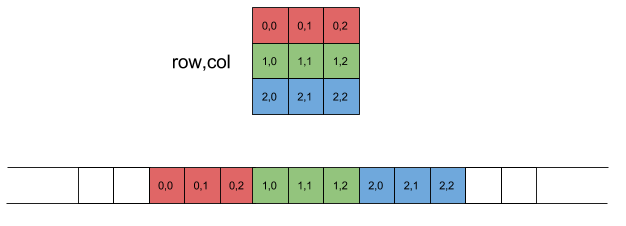
\includegraphics[scale=0.6]{./figures/2_tnv/row-major-2D}
\end{center}

\newpage \noindent Αντίθετα μία κατά στήλες (column-major) αναπαράσταση του μητρώου στην μνήμη θα ήταν η αντίστοιχη: 

\begin{center}
    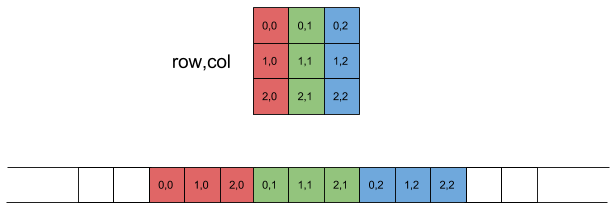
\includegraphics[scale=0.6]{./figures/2_tnv/column-major-2D}
\end{center} 

Σε κάθε περίπτωση εμείς στην υλοποίησή μας διαθέτουμε τα δεδομένα μας στην εξής μορφή:

\begin{center}
    Matrix A = 
\begin{pmatrix} 
0 & 1 & 2 \\
3 & 4 & 5 \\
6 & 7 & 8
\end{pmatrix}
\hspace{0.5cm}Matrix A\textsuperscript{T} =
\begin{pmatrix} 
0 & 3 & 6 \\
1 & 4 & 7 \\
2 & 5 & 8
\end{pmatrix}

\vspace{0.4cm}

{\large \texttt{A[] = \{0, 1, 2, 3, 4, 5, 6, 7, 8\}}}

\end{center}

Έτσι λοιπόν προκειμένου να αποφύγουμε την διπλή αποθήκευση του μητρώου στην μνήμη, εκμεταλλευόμαστε την παρουσία του Α ώστε διατρέχοντας το με τον κατάλληλο τρόπο να προσπευλαύνουμε το ανάστροφό του. Η πρακτική αυτή συνδέεται στενά με την έννοια του coalescing που περιγράφεται παρακάτω.



\subsection*{Memory Coalescing / Row-Major \& Column-Major Traversal}
\addcontentsline{toc}{subsection}{Memory Coalescing / Row-Major \& Column-Major Traversal}


\begin{center}
    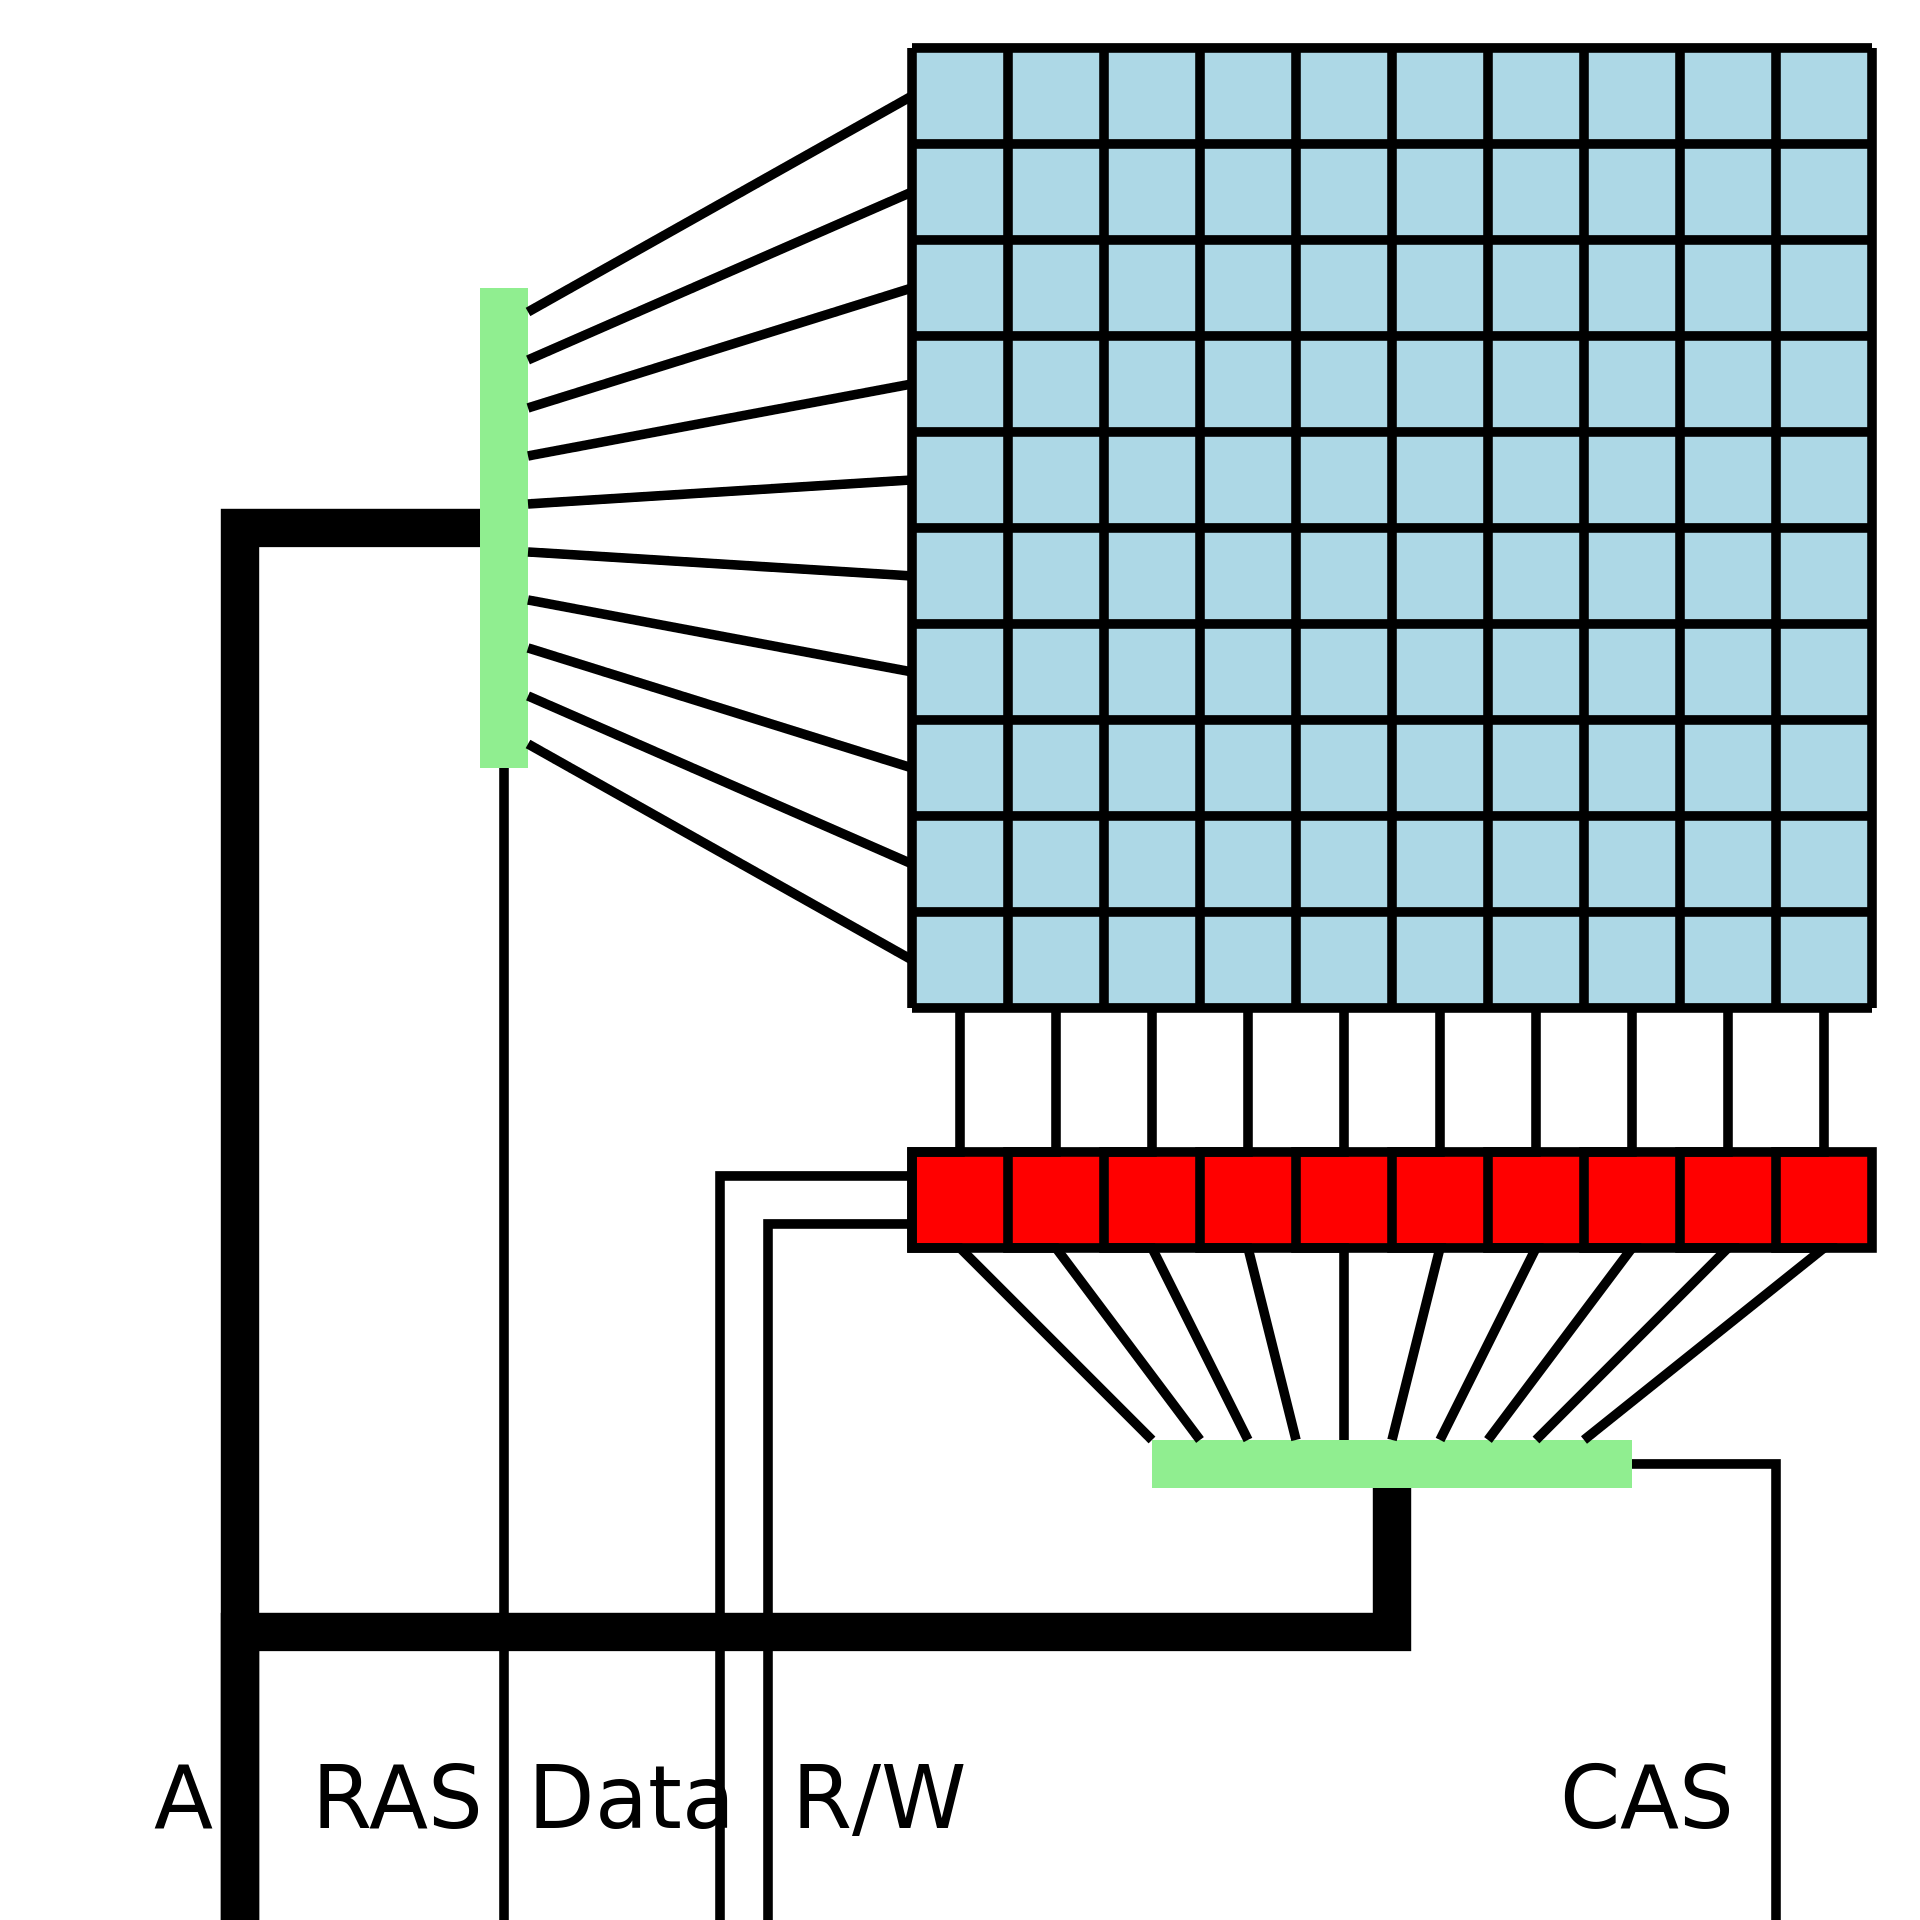
\includegraphics[scale=0.1]{./figures/2_tnv/DRAM}
    
    {\small \textit{Τυπική αρχιτεκτονική DRAM bank}}
\end{center}

Εξ αιτίας της κατασκευής των DRAM, όπου ο τρισδιάστατος, οργανωμένος σε banks φυσικός χώρος διευθύνσεων, αντιστοιχίζεται σε έναν γραμμικό λογικό χώρο, όταν προσπελαύνεται μία θέση μνήμης στην πραγματικότητα γίνονται διαθέσιμα τα δεδομένα περισσότερων από μία διαδοχικών διευθύνσεων.
Λαμβάνοντας υπόψιν ότι όλα τα thread σε ένα warp εκτελούν την ίδια εντολή, αν οργανώσουμε τον κώδικα μας με τέτοιο τρόπο ώστε τα threads κάθε χρονική στιγμή να προσπελαύνουν συνεχόμενες θέσεις μνήμης τότε εκμεταλλευόμενοι την παραπάνω συμπεριφορά μπορούμε να πετύχουμε σημαντική βελτίωση της επίδοσης του προγράμματός μας. Η τεχνική αυτή ονομάζεται memory coalescing \cite{Harris:coal}. Ας εξετάσουμε το παρακάτω παράδειγμα:


\begin{verbatim}
2D array:                   1D mapping in memory:
0  1  2  3                  0 1 2 3 4 5 6 7 8 9 a b
4  5  6  7                  element (r,c) maps to (r*4+c)
8  9  a  b

row-major traversal:                        column-major traversal:
thread 0:  0, 1, 2                          thread 0:  0, 4, 8
thread 1:  3, 4, 5                          thread 1:  1, 5, 9
thread 2:  6, 7, 8                          thread 2:  2, 6, a
thread 3:  9, a, b                          thread 3:  3, 7, b
----------time---------->                   ----------time---------->
\end{verbatim}

Θεωρούμε ότι έχουμε ένα 3Χ4 μητρώο αποθηκευμένο στην μνήμη σειριακά, με οργάνωση κατά γραμμή. Αν επίσης διαθέτουμε 4 thread καθένα εκ των οποίο σε κάθε βήμα προσπελαύνει μία θέση του πίνακα, τότε κάθε thread θα αναλάβει συνολικά την επεξεργασία τριών στοιχείων. Αν λοιπόν σε κάθε thread αντιστοιχήσουμε τα στοιχεία που του αναλογούν με έναν row-major τρόπο τότε κάθε χρονική στιγμή θα καταλήξουν να μην προσπελαύνουν διαδοχικές θέσεις μνήμης. Αντίθετα αν κάθε thread κινείται στα στοιχεία μιας στήλης (column-major traversal) τότε θα πετύχουμε το επιθυμητό αποτέλεσμα. Η συμπεριφορά αυτή γίνεται πιο εύκολα κατανοητή παρατηρώντας το παρακάτω σχήμα στο οποίο αριστερα απεικονίζονται οι θέσεις μνήμης που προσπελαύνουν τα 4 threads, στο πρώτο βήμα του υπολογισμού, αν χρησιμοποιείται row-major traversal ενω δεξιά η αντίστοιχη συμπεριφορά για column-major traversal.

%\begin{center}
    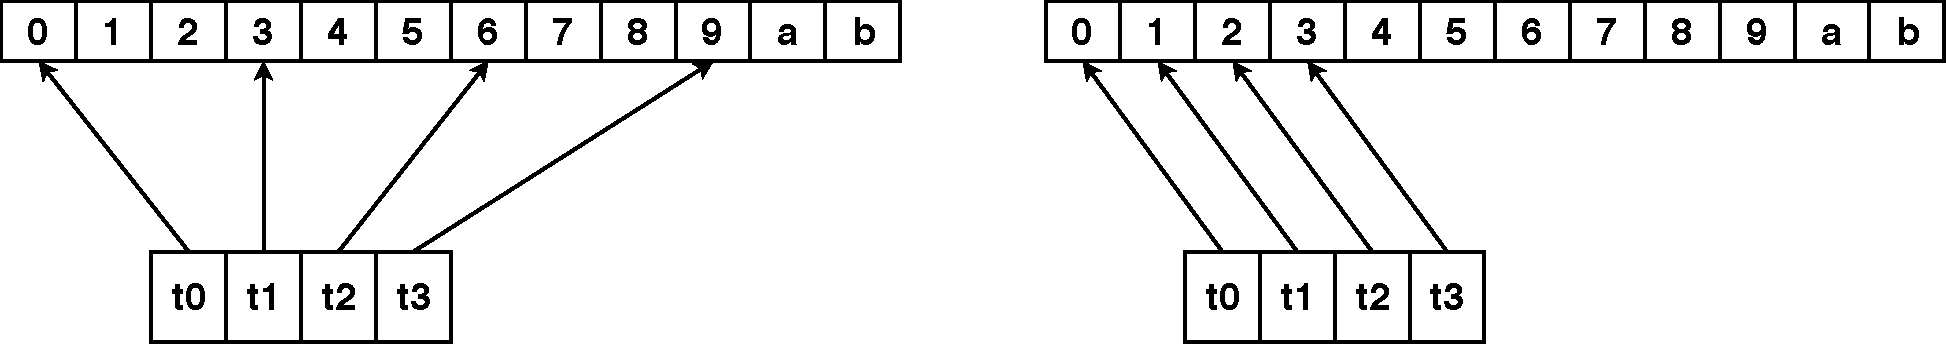
\includegraphics[scale=0.45]{./figures/2_tnv/coal.pdf}
%\end{center}

Η αξιοποίηση αυτής της τεχνικής βρίσκει άμεση εφαρμογή στο πρόβλημά μας κατά τον πολλαπλασιασμό του μητρώου A\textsuperscript{T} με το διάνυσμα (Ax). Εξαιτίας του τρόπου με τον οποίο έχουμε αποθηκευμένο το μητρώο στην μνήμη, διατρέχοντας τα στοιχεία του Α υποθέτοντας οργάνωση κατά στήλες ουσιαστικά επιτυγχάνουμε την προσπέλαση του ανάστροφού του με coalesced τρόπο. 

\subsection*{Shared Memory}
\addcontentsline{toc}{subsection}{Shared Memory}

\noindent Η προσπέλαση της shared memory είναι αρκετές τάξεις μεγέθους ταχύτερη σε σχέση με αυτήν της global memory επομένως μπορούμε να την αξιοποιήσουμε για να βελτιώσουμε την απόδοση της εφαρμογής μας. Βέβαια με τη χρήση της προκύπτουν δύο ζητήματα που πρέπει να λάβουμε υπόψιν. Αρχικά πρέπει να μεταφέρουμε στην κοινόχρηστη μνήμη μόνο τα δεδομένα που θα χρησιμοποιηθούν παραπάνω από μία φορές (ιδανικά πολλές περισσότερες) καθώς και να τροποποιήσουμε τον αλγόριθμό μας ώστε να τα χρησιμοποιεί σε μία φάση ώστε να αποφύγουμε τις εναλλασσόμενες μεταφορές των ίδιων στοιχείων. Σε περίπτωση που ένα στοιχείο χρησιμοποιείται μόνο μία φορά είναι ανώφελο να το μεταφέρουμε στην shared memory καθώς στην πράξη θα προσθέσουμε επιπλέον επιβάρυνση για τη μεταφορά και τη χρήση του.

Επίσης η shared memory είναι διαθέσιμη σε επίπεδο block. Δηλαδή μόνο τα threads του ίδιου block έχουν πρόσβαση στα κοινά δεδομένα. Το δεύτερο ζήτημα που προκύπτει είναι ότι κάθε block έχει διαθέσιμα \mbox{49152 bytes} (48KB) κοινόχρηστης μνήμης με αποτέλεσμα να πρέπει να είμαστε προσεκτικοί να μην ξεπεράσουμε το όριο αυτό. Στον δικό μας αλγόριθμο εφαρμόζουμε τη χρήση της shared memory κατά τον πολλαπλασιασμό μητρώου διανύσματος.

\newpage

\subsection*{Σύνοψη υλοποίησης}
\addcontentsline{toc}{subsection}{Σύνοψη υλοποίησης}

Η υλοποίηση μας αποτελείται από δύο υπολογιστικούς πυρήνες (kernels):
\begin{enumerate}
    \item \textbf{\texttt{\textunderscore\textunderscore global\textunderscore\textunderscore\ void matvec\textunderscore kernel\textunderscore row\textunderscore major(...)}}
    
    Στον kernel αυτόν υλοποιείται η πράξη του πολλαπλασιασμού μητρώου διανύσματος και χρησιμοποιείται για την εκτέλεση της πρώτης πράξης, δηλαδή της $(Ax)$. Για την προσπέλαση των στοιχείων του διανύσματος x γίνεται χρήση της shared memory καθώς τα στοιχεία του χρησιμοποιούνται με μεγαλύτερη συχνότητα και επαναλαμβανόμενα για τον υπολογισμού του αποτελέσματος. Το μητρώο Α βρίσκεται αποθηκευμένο στην global memory και κάθε thread πραγματοποιεί προσπέλαση στοιχείων με row-major τρόπο (υποθέτοντας οργάνωση στη μνήμη κατά γραμμές), με αποτέλεσμα οι προσπελάσεις της global memory να μην ειναι coalesced.
    
    Για την κλήση του υπολογιστικού πυρήνα έχει δημιουργηθεί μία συνάρτηση-wrapper η οποία αναλαμβάνει να υπολογίσει το απαιτούμενο grid size ανάλογα το μέγεθος του προβλήματος, την κλήση του kernel καθώς και την χρονομέτρησή του. Η συνάρτηση αυτή είναι η: \textbf{\texttt{\textunderscore\textunderscore host\textunderscore\textunderscore\  float matvec\textunderscore ROW\textunderscore MAJOR(...)}}
    
    
    
     %\newpage
     
     
    \item \textbf{\texttt{\textunderscore\textunderscore global\textunderscore\textunderscore\ void matvec\textunderscore kernel\textunderscore column\textunderscore major(...)}}
    
    Στον kernel αυτόν υλοποιείται η πράξη του πολλαπλασιασμού μητρώου διανύσματος και χρησιμοποιείται για την εκτέλεση της πρώτης πράξης, δηλαδή της $A^{T}(Ax)$ όπου το $(Ax)$ πλέον αποτελεί ένα διάνυσμα ως το αποτέλεσμα της προηγούμενης πράξης. Για την προσπέλαση των στοιχείων του διανύσματος x γίνεται χρήση της shared memory καθώς τα στοιχεία του χρησιμοποιούνται με μεγαλύτερη συχνότητα και επαναλαμβανόμενα για τον υπολογισμού του αποτελέσματος. Το μητρώο Α βρίσκεται αποθηκευμένο στην global memory και κάθε thread πραγματοποιεί προσπέλαση στοιχείων με column-major τρόπο, υποθέτωντας οργάνωση στη μνήμη κατά στήλες, ώστε να γίνεται η πράξη με το ανάστροφο του μητρώου Α. Αυτό έχει ως αποτέλεσμα οι προσπελάσεις της global memory να ειναι coalesced. 
    
    Αντίστοιχα έχει δημιουργηθεί η συνάρτηση-wrapper:
    \textbf{\texttt{\textunderscore\textunderscore host\textunderscore\textunderscore\  float matvec\textunderscore COL\textunderscore MAJOR(...)}}
\end{enumerate}

\subsection*{cuBLAS - gemv}
\addcontentsline{toc}{subsection}{cuBLAS - gemv}

\noindent Προκειμένου να αξιολογήσουμε την απόδοση της δικής μας υλοποίησης αποφασίσαμε να δοκιμάσουμε την εκτέλεση των ίδιων πράξεων με χρήση της υλοποίησης της BLAS που παρέχει η CUDA, δηλαδή την cuBLAS. Συγκεκριμένα με χρήση της level 2 συνάρτησης gemv (generalized matrix vector multiplication) εκτελέσαμε τους πολλαπλασιασμούς μητρώου-διανύσματος όπου απαιτούνται.


\subsection*{Αποτελέσματα}
\addcontentsline{toc}{subsection}{Αποτελέσματα}

\noindent Παρακάτω παρατίθενται οι μέσοι χρόνοι όπως προέκυψαν μετά την εκτέλεση του προγράμματος 10 φορές για κάθε διαφορετικό μέγεθος εισόδου. Το μέγεθος σε MByte που αναφέρεται αφορά μόνο τον χώρο που καταλαμβάνει στη μνήμη το μητρώο Α και αποτελεί μία ένδειξη του μεγέθους του προβλήματος.

\begin{center}
    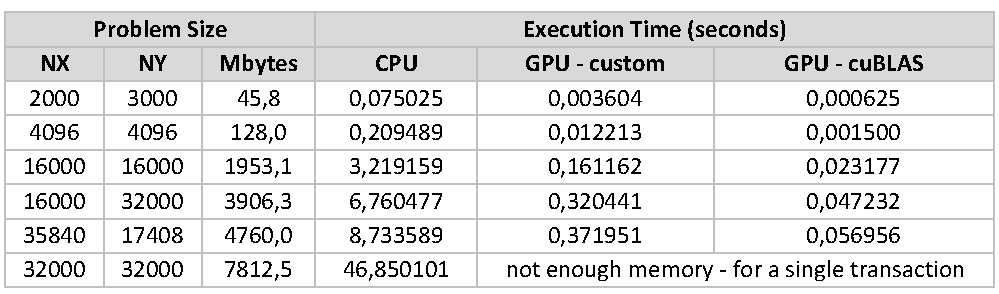
\includegraphics[scale=0.9]{./figures/2_tnv/new1}
\end{center}

\newpage
\noindent Στον πίνακα που ακολουθεί αναλύονται οι χρόνοι εκτέλεσης του υπολογισμού ανα kernel για τα διάφορα μεγέθη εισόδου:

\begin{center}
    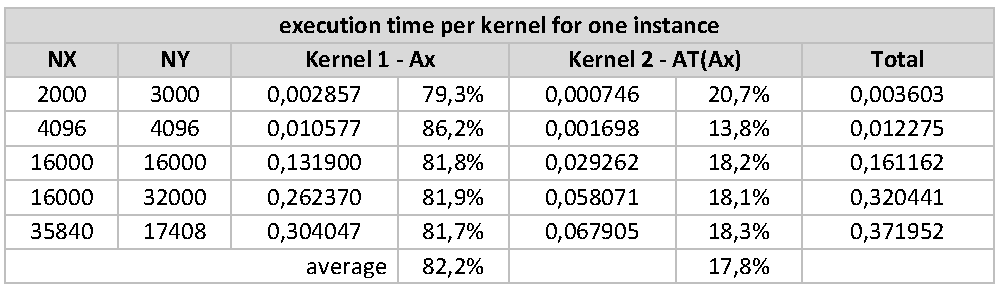
\includegraphics[scale=0.9]{./figures/2_tnv/new2}
\end{center}

\subsection*{Συμπεράσματα}
\addcontentsline{toc}{subsection}{Συμπεράσματα}

\begin{center}
    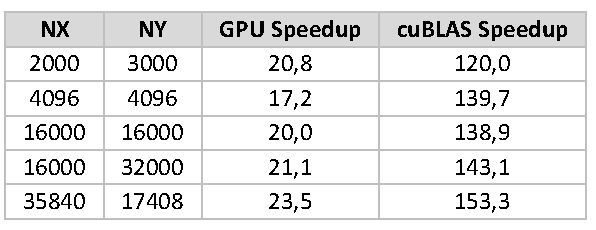
\includegraphics[scale=0.9]{./figures/2_tnv/speed_new}
\end{center}

\noindent Υπολογίζοντας τα μετρούμενα speedup τόσο της υλοποίησής μας όσο και της cuBLAS μπορούμε να οδηγηθούμε σε κάποια συμπεράσματα. Αρχικά ενώ έχουμε καταφέρει να πάρουμε αρκετά καλή βελτίωση της απόδοσης μέσω της δικής μας υλοποίησης γίνεται φανερό ότι χρήση της cuBLAS σε μία πιθανή εφαρμογή θα ήταν επιβεβλημένη, καθώς επιτυγχάνει εξαιρετική επιτάχυνση, ``εκτός ανταγωνισμού''.

\noindent Μπορούν να γίνουν οι εξής παρατηρήσεις:

\begin{enumerate}
    \item Όταν οι διαστάσεις του μεγέθους του μητρώου Α αποτελούν δυνάμεις του 2 ή πολλαπλάσια τους τότε έχουμε καλύτερα αποτελέσματα, από την άποψη μας ότι ο αλγόριθμος μας είναι πιο αποδοτικός. Ένας λόγος για τον οποίο μπορεί να συμβαίνει αυτό είναι ότι δημιουργούνται ομοιόμορφα grid και blocks στα οποία όλα τα thread αναλαμβάνουν αξιοποιούνται για τον υπολογισμό με αποτέλεσμα το μεγαλύτερο occupancy.
    
    \item Παρατηρούμε ότι ο δεύτερος kernel είναι σημαντικά ταχύτερος καθώς καταλαμβάνει μόνο το 10\% του συνολικού χρόνου κατά μέσο όρο, αν και φαινομενικά εκτελεί τον ίδιο υπολογισμό. Αυτό συμβαίνει καθώς πέρα από την χρήση της shared memory για την αποθήκευση του διανύσματος x εκμεταλλεύεται και την τεχνική του coalescing όταν προσπελαύνει τα στοιχεία του Α\textsuperscript{T} από την global memory.
\end{enumerate}


\subsection*{Περαιτέρω Βελτίωση}
\addcontentsline{toc}{subsection}{Περαιτέρω Βελτίωση}

\noindent Είναι φανερό ότι υπάρχουν μεγάλα περιθώρια βελτίωσης της απόδοσης της εφαρμογής μας τα οποία όμως ίσως ξεφεύγουν από τα πλαίσια της παρούσας εργασίας. Θα μπορούσαμε να τα συνοψίσουμε στα εξής σημεία:

\begin{itemize}
    \item Θα πρέπει να επικεντρωθούμε στην βελτίωση του πρώτου υπολογιστικού πυρήνα ο οποίος προσπελαύνει την global memory με μη-coalesced τρόπο με αποτέλεσμα την σημαντική επιβάρυνση του απαιτούμενου χρόνου. Μια ιδέα είναι να μεταφέρουμε τμήματα του μητρώου Α στην shared memory κατα την διάρκεια του υπολογισμού υλοποιώντας ουσιαστικά έναν \textbf{tiled shared memory} αλγόριθμο πολλαπλασιασμού μητρώου διανύσματος. Μία τέτοια προσέγγιση προτείνεται στην εργασία \cite{Erik:tiled}, την οποία αν και καταφέραμε και εντάξαμε στην υλοποίηση μας με πολύ καλά αποτελέσματα για τετραγωνικά μητρώα με διαστάσεις δυνάμεις του 2, δεν δούλευε για όλα τα μεγέθη εισόδου. Μια λύση θα ήταν να τροποποιήσουμε τον κώδικά μας ώστε να μετατρέπει το μητρώο εισόδου σε τετραγωνικό με μέγεθος κάθε διάστασης την κοντινότερη δύναμη του 2 για την μεγαλύτερη από τις 2 αρχικές.
    
    \item Το δεύτερο σημείο επικεντρώνεται στην παρατήρηση οτι η cuBLAS επιτυγχάνει εξαιρετικά αποτελέσματα. Καθώς πρόκειται για μια closed source βιβλιοθήκη της nVidia δεν έχουμε πρόσβαση στον κώδικα της ώστε να προσπαθήσουμε τον κατανοήσουμε τον τρόπο λειτουργίας της. Για τον λόγο αυτό αναζητήσαμε να βρούμε open source υλοποιήσεις της BLAS για GPU και να δούμε με ποιον τρόπο αντιμετωπίζουν την gemv. Πράγματι εντοπίσαμε την \href{https://github.com/ecrc/kblas-gpu/}{kblas-gpu} η οποία υλοποιεί τις \href{https://github.com/ecrc/kblas-gpu/tree/master/src/blas_l2}{level 2} συναρτήσεις της blas. Αν είχαμε περισσότερο χρόνο θα μπορούσαμε να μελετήσουμε και αυτήν την προσέγγιση για να δούμε αν θα πετυχαίναμε περαιτέρω βελτίωση.
    
    % \item Μία ακόμα ιδέα βελτιστοποίησης που προέκυψε τελευταία στιγμή είναι αντί να αντιμετωπίσουμε τον  πρώτο υπολογισμό ως έναν πολλαπλασιασμό
\end{itemize}

% Μία ιδέα βελτιστ

% \begin{center}
%     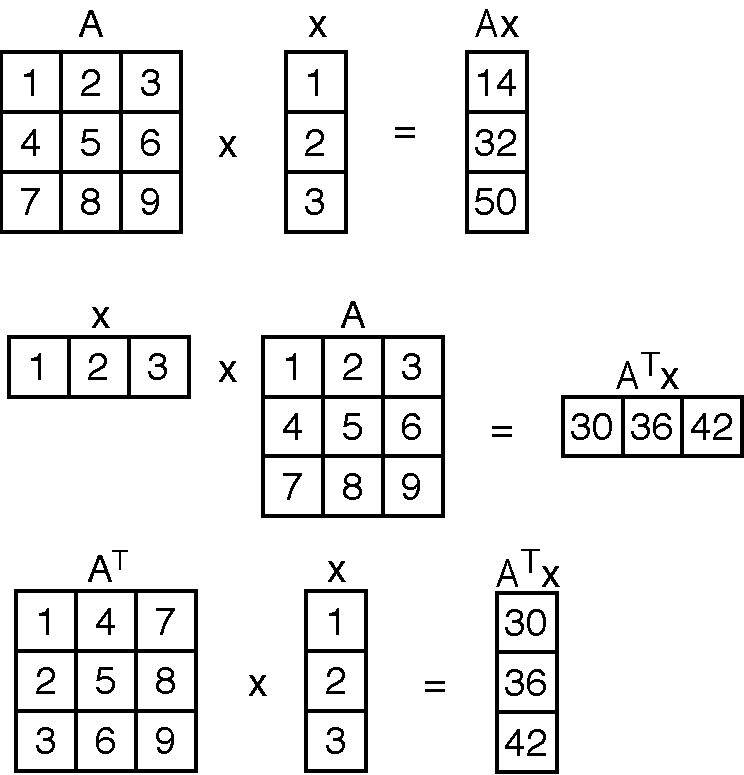
\includegraphics[scale=0.8]{./figures/2_tnv/mult}
% \end{center}


\newpage